\clearpage
\section*{\currfilename}

\begin{figure}[H]
  \fontsize{10pt}{10pt}\selectfont
  \begin{center}
    \begin{tikzpicture}[auto, scale=1.0, every node/.style={transform shape}, node distance=1.0cm, >=latex']
      \node[squareblock, minimum height=1cm, minimum width=2cm] (block1){\shortstack[c]{Baseline\\Control}};
      \node[squareblock, below of=block1, node distance=1.5cm, minimum height=1cm, minimum width=2cm] (block2){\shortstack[c]{Adaptive\\Augmentation}};

      \node[coordinate,below of=block1, node distance=0.75cm] (node1) {};
      \node[coordinate,right of=node1, node distance=1.5cm] (node_control) {};
      \node[coordinate,left of=node1, node distance=1.5cm] (node_reference) {};
      \node[coordinate, left of=node_reference, node distance=1.5cm] (node_input) {};
      \node[coordinate, right of=node_input, node distance=0.5cm] (node_tee1) {};
      \node[coordinate, below of=block3, node distance=2.5cm] (node_tee2) {};

      \node[right of=node_control,draw=black, node distance=3.5cm, minimum width=2cm, inner sep= 0mm] (block3) {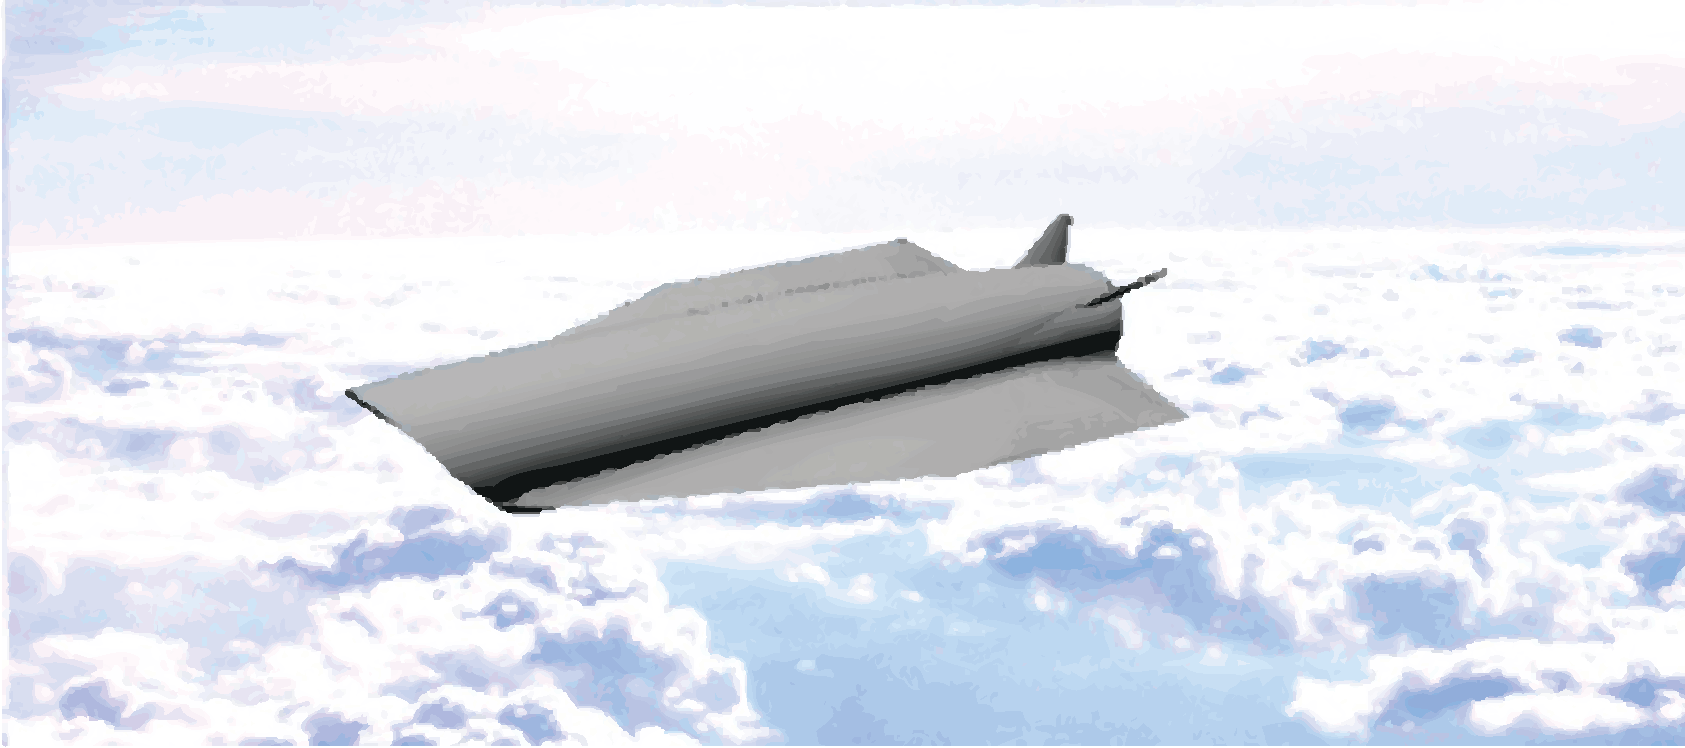
\includegraphics[width=4cm]{../fig/ghvclouds.pdf}};
      \node[squareblock, minimum height=1.5cm, minimum width=4.0cm, above of=block3,node distance=2.25cm] (block4) {\shortstack[c]{Reference\\Model}};
      \node[whitesum,right of=block3, node distance=3.5cm] (sum2) {};
      % \node[coordinate,above of=sum2, node distance=3.5cm] (node_L) {};
      % \node[squareblock, minimum height=1.0cm, minimum width=1.0cm, above of=sum2,node distance=3.5cm] (block_L) {$L$};

      \node[input,below of=block2, node distance=1.5cm] (input2) {};
      \node[coordinate,right of=sum2, node distance=0.25cm] (node_output) {};
      \node[output,right of=node_output, node distance=1.5cm] (output1) {};
      \node[coordinate,below of=block3, node distance=2.5cm] (node_feedback) {};
      \node[coordinate,left of=node_feedback, node distance=1.5cm] (node_feedback2) {};
      \node[coordinate,below of=block2, node distance=0.7cm] (node_feedback3) {};

      % Gray shaded box
      \begin{pgfonlayer}{background}
        \path (block1 |- block1)+(-1.5,0.7) node (c) {};
        \path (block2 -| block2)+(1.5,-0.7) node (d) {};
        \path[fill=gray!20, draw] (c) rectangle (d);
      \end{pgfonlayer}

      % Draw
      \draw [vecArrow]  (node_control) -- (block3);
      \draw [vecArrow]  (node_tee1) |- (block4);
      \draw [vecArrow]  (node_input) -- (node_reference);
      \draw [vecArrow]  (block3) -- node [pos=0.7]{$+$} (sum2);
      \draw [vecArrow]  (block4) -| node [pos=0.9]{$-$} (sum2);
      % \draw [vecArrow]  (node_output) |- (block_L);
      \draw [vecArrow]  (sum2) -- (output1);
      \draw [vecNoArrow]  (block3) |- (node_feedback2);
      \draw [vecArrow]  (node_feedback2) -| (node_feedback3);

      % \draw [vecArrow]  (block_L) -| (block4);
      % \draw [->]  (b1inB) + (-0.5cm,0cm) -> (b1inB);
      % \draw [->]  (b2inA) + (-1cm,0cm) -> (b2inA);
      % \draw [->]  (b2inB) + (-2.0cm,0cm) -> (b2inB);
      % \draw [-]  (b2inB) + (-2.0cm,0cm) |- (input2);
      % \draw[->](block3) --  node[name=yi,pos=0.3]{state} node[pos=0.9]{$+$} (sum2);
      % \draw[-](yi) |- (input2);

      % \draw [-]  (b1inBleft) + (0.0cm,-1.5cm) -- (b1inBleft);
      % \draw [-]  (b2inAleft) + (0.0cm,1.5cm) -- (b2inAleft);
      % \draw[->](block1) -- node[pos=0.7]{$+$} (sum1);
      % \draw[->](block2) -| node[pos=0.9]{$+$} (sum1);
      % \draw[->](sum1) -- node[pos=0.6]{control} (block3);
      % \draw[->](block4) -| node[pos=0.1]{reference} node[pos=0.95]{$-$} (sum2);
      % \draw[->](sum2) -- node[pos=0.4]{error} (output1);
    \end{tikzpicture}
  \end{center}
\end{figure}
